\documentclass{scrartcl}

\KOMAoption{toc}{bibliography}
\KOMAoptions{
	paper=a4,
	fontsize=12pt,
	parskip=true,
	titlepage=false,
	%appendixprefix=true,
	%abstract=true,
}
\addtokomafont{disposition}{\boldmath}

% section numbering
%\renewcommand*{\thesection}{\thepart.\arabic{section}}
%\DeclareTOCStyleEntry[numwidth=0.85cm]{tocline}{section}

\usepackage{fontspec} % find out what this package does exactly
\setmainfont{FreeSerif}
\setsansfont{FreeSans}
% URLs should (still) be typed using monospace font
% https://graphicdesign.stackexchange.com/questions/97173/is-monospacing-urls-in-academic-papers-still-advised
\setmonofont{FreeMono}
%\newfontfamily\DejaSans{DejaVu Sans} % to display emojis

\usepackage{csquotes} % quotation marks
\usepackage[onehalfspacing]{setspace}
\usepackage{mathtools}
\usepackage[english,german]{translator} % siunitx needs translator package (not ngerman)! 
\usepackage{siunitx}[=v2]
\sisetup{%
	separate-uncertainty=true,
	%mode=match
	%locale=?
	%per-mode=fraction,
}
\DeclareSIUnit\ppm{\text{ppm}}
\DeclareSIUnit\year{\text{yr}}
\NewDocumentCommand{\angsi}{omom}{%
	\ang[#1]{#2}\,\si[#3]{#4}%
}
% https://tex.stackexchange.com/questions/116426/recommend-way-to-get-angular-velocity-in-degree-with-siunitx
\usepackage[
pdfauthor={Robert Wright},
%pdftitle={},
]{hyperref}
\hypersetup{
	colorlinks=true,
	urlcolor=.,
	linkcolor=,
	citecolor=,
}
\usepackage{graphicx}
\usepackage{wrapfig}
\usepackage{float}
\usepackage{pdfpages}
\usepackage{caption}
\usepackage{subcaption}
\usepackage{cleveref}
\usepackage{booktabs, makecell}
%\usepackage{tabularx}
\usepackage[roman]{parnotes}
\usepackage[shortcuts]{extdash} % to hyphenate words with dashes in them
%\usepackage{parskip} % not needed anymore as koma script provides this function
\usepackage{xcolor}
\usepackage[enable]{easy-todo}
\usepackage[version=4]{mhchem}

% LANGUAGE & DATE
% Note: In general, it is advisable to activate the languages
%       after all packages have been loaded
\usepackage{polyglossia}
\setdefaultlanguage[variant=british]{english}
\setotherlanguages{ngerman}
% load datetime2 after language is set
% (can’t detect the region with polyglossia)
\usepackage[en-GB]{datetime2}
\DTMlangsetup[en-GB]{ord=raise}

% REFERENCES
\usepackage[
	backend=biber,
	style=numeric,
	%bibstyle=authortitle,
	autolang=langname,
	uniquename=init,
	giveninits=true,
	maxnames=2,
	%block=ragged,
	%sorting=none,
]{biblatex}
\addbibresource{lit.bib}
% don't print url and urldate
%\AtEveryBibitem{
%	\clearfield{url}
%	\clearfield{urlyear}
%}

%%%%%%%%%%%%%%%%%%%%%%%%%%%%%%%%%%%%%%%%%%%%%%%%%%%%%%%%%%%%%%%%%%%%%%%%%%%%%%%%%%%
% https://tex.stackexchange.com/questions/16765/biblatex-author-year-square-brackets
\makeatletter

\newrobustcmd*{\parentexttrack}[1]{%
	\begingroup
	\blx@blxinit
	\blx@setsfcodes
	\blx@bibopenparen#1\blx@bibcloseparen
	\endgroup}

\AtEveryCite{%
	\let\parentext=\parentexttrack%
	\let\bibopenparen=\bibopenbracket%
	\let\bibcloseparen=\bibclosebracket}

\makeatother
%%%%%%%%%%%%%%%%%%%%%%%%%%%%%%%%%%%%%%%%%%%%%%%%%%%%%%%%%%%%%%%%%%%%%%%%%%%%%%%%%%%
% COSTUM COMMANDS

% change figsize globally
\newcommand{\figwidth}{\textwidth}

\newcommand{\kopf}[1]{%
	\Large\textsf{\textbf{#1}}
}

% Markdown code style
\definecolor{light-gray}{gray}{0.95}
\newcommand{\code}[1]{\colorbox{light-gray}{\texttt{#1}}}

% math stuff
\newcommand*\mean[1]{\overline{#1}}
\newcommand{\vect}[1]{\boldsymbol{#1}}

% chemnistry stuff
\newcommand{\co}{\ce{CO2}}

%%%%%%%%%%%%%%%%%%%%%%%%%%%%%%%%%%%%%%%%%%%%%%%%%%%%%%%%%%%%%%%%%%%%%%%%%%%%%%%%%%%
% TITLE

\subject{\textngerman{Modelle für Wetter \& Umwelt}}
\title{COSMO-CLM: Influence of Grid Resolution on Precipitation Forecast}
%\subtitle{}
\author{Robert Wright}
\date{\DTMdisplaydate{2023}{7}{24}{-1}}

%%%%%%%%%%%%%%%%%%%%%%%%%%%%%%%%%%%%%%%%%%%%%%%%%%%%%%%%%%%%%%%%%%%%%%%%%%%%%%%%%%%

\begin{document}
	
	\maketitle
	%\tableofcontents 
	% https://tex.stackexchange.com/questions/341613/komascript-toc-prevent-column-break-between-sections-in-multicolumn-toc
	
	%\input{sections/abstract.tex}
	\section{Introduction}

In 1952, the \textit{Met Office}, i.e., the UK's national weather service, successfully completed its first numerical weather prediction forecast on a 12 \(\times\) 8 grid with grid point spacing of \SI{260}{\km} \parencite{MetOffice}. Since then, weather forecasts have improved tremendously, not least because of an increase in grid resolution. This development has been made possible by the continued growth of available computational power. While, on the one hand, increased grid resolution undoubtedly improved the numerical weather forecast, on the other hand, it also increased the need for adequate computational resources. The CFL criterion introduces an upper limit for the time step proportional to the grid point separation---a high grid resolution thus demands a short time step, which is computationally more expensive. Therefore, it is of interest to understand the influence of grid resolution on numerical weather prediction in order to find the best compromise of grid point spacing in terms of computing time and forecast quality. 
% hier fehlt irgendwie noch ein Satz, dass mein Projekt natürlich zu klein ist um diese Frage wirklich zu beantworten
In this study, a regional weather model calculates one-month forecasts on three different spatial resolutions for the region of Europe. Then, the change in precipitation patterns due to varying grid size is analysed. Generally speaking, precipitation plays a major role in weather forecasts, hence, it seems natural to use this variable in order to compare grid resolution. On top, as a diagnostic variable, it is based on multiple direct model predictions and captures the effects of resolution-dependent internal model dynamics.
	\section{Model setup \& data}

The \textbf{C}OSMO model in \textbf{CL}imate \textbf{M}ode (CCLM) is the climate version of the COSMO model, that has been designed for operational mesoscale numerical weather prediction. CCLM, as a limited-area atmospheric model, receives boundary and initial conditions from a driving host model, or, in our case study, from ERA-Interim reanalysis data (resolution of 0.75°). Time integration relies on a third-order Runge-Kutta scheme. The number of both vertical and soil levels is equal to 10. The model equations are formulated in rotated geographical coordinates to reduce the effect of varying grid cell size. Parametrization for grid-scale clouds and precipitation is based on a Kessler-type bulk formulation, which uses specific grouping of particles into broad categories of water substance (e.g., cloud water) that interact by various microphysical processes. The implemented cloud ice scheme allows explicit representation of ice clouds. While vertical turbulent diffusion parametrization is based on a prognostic equation for turbulent kinetic energy, as far as I am concerned, no subgrid-scale (deep) convection scheme is included by default\footnote{\code{itype\_conv} undefined in model namelists}.   
The time step has been set to \SI{150}{\s} for all grid resolutions. For further information about the COSMO model please refer to \textcite{schaettler2021}.

\begin{table}[h]
	\centering
	\begin{tabular}{cccc}
		\toprule
		Experiment name & Resolution [°] & Grid & Spacing [\(\approx\)km] \\
		\midrule
		02° & 0.2 & 280 \(\times\) 230 & 25 \\
		05° & 0.5 & 100 \(\times\) 80  & 65 \\
		1° & 1 & 56 \(\times\) 46      & 130 \\
		\bottomrule
	\end{tabular}
	\caption{CCLM simulations of this study}
	\label{tab:sims}
\end{table}

The study is composed of three CCLM simulations during January 1990, as introduced in \cref{tab:sims}. This period of time has been chosen as grid definition files and appropriately scaled boundary conditions were already available. \Cref{fig:regionbox} displays the mean precipitation within the entire model domain, however, structures of \enquote{unphysical} values are clearly visible at the edges, where interpolation between model predictions and constraining boundary conditions distorts the results. In the following, the region of interest is reduced to the area within the red rectangle in \cref{fig:regionbox}. It is notable that the 05°-simulation region seems to be cropped in the north and east compared to the other simulations. This is due to an erroneous value in the number of grid points during grid definition, but will not affect the results as the region of analysis is still sufficiently large. 

\begin{figure}[h]
	\centering
	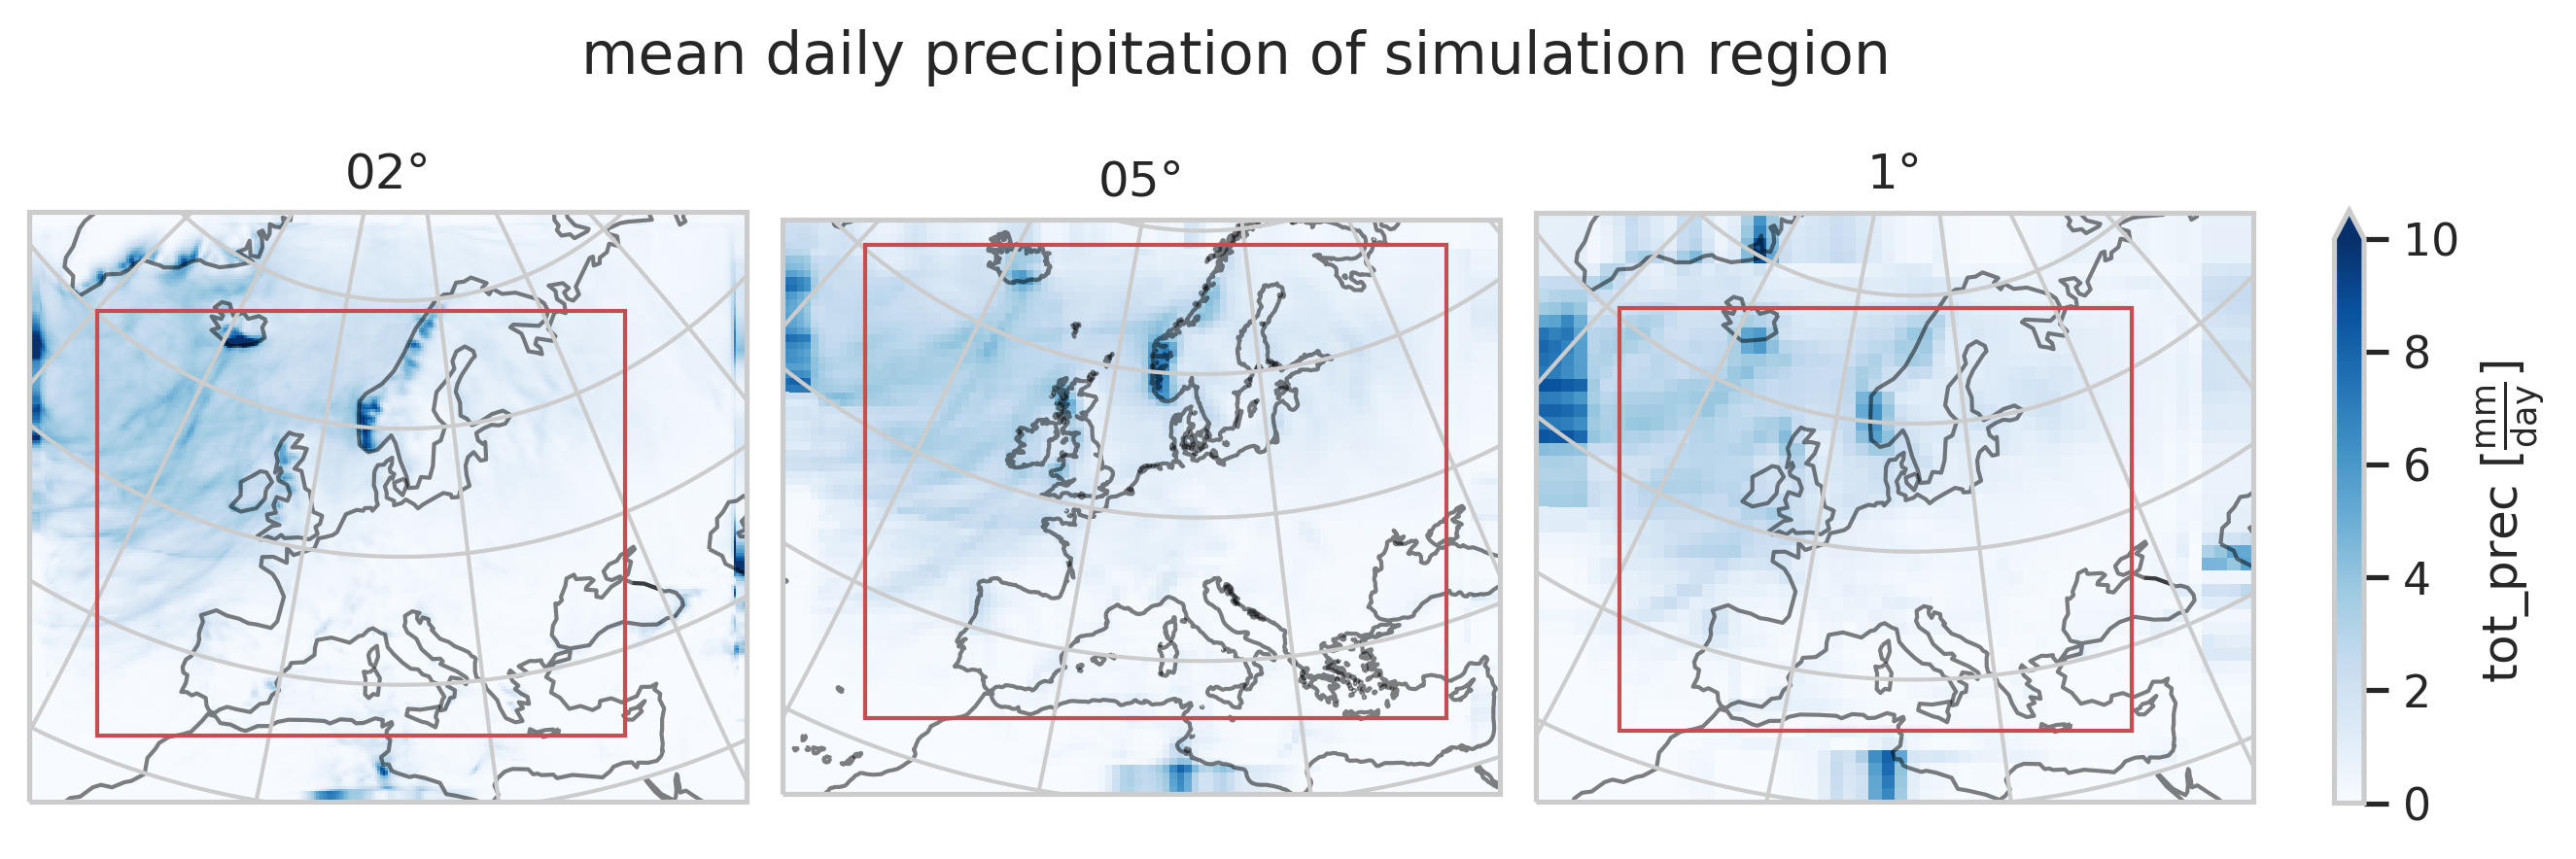
\includegraphics[width=\figwidth]{../figs/1-regionbox.png}
	\caption{Spatial domains of simulations. Red rectangle indicates area of analysis. Please note that here and in the following figures pointed ends of a colourbar indicate existing out-of-range values.}
	\label{fig:regionbox}
\end{figure}
	
In this study, ERA5 reanalysis data produced by the ECMWF serves as a reference. Although also a model product themselves, reanalyses assimilate observational records and thus are a reasonable choice to compare simulation output against. ERA5 data is provided on a 0.28° grid, however, the data is remapped to a 0.2° rotated grid to be able to cut the same region as in the CCLM simulations (see \cref{fig:regionbox}).

The shell script for data processing, python code for re-creating all figures as well as further comments can be found in the corresponding online repository\footnote{\url{https://gitlab.met.fu-berlin.de/rw0064fu/mwu-gridres}}. Much data processing has been realized by using \textit{Climate Data Operators} of \textcite{schulzweida2022}. 
	%\input{sections/methods.tex}
	\section{Results}

% was erzähle ich hier?

\begin{figure}
	\centering
	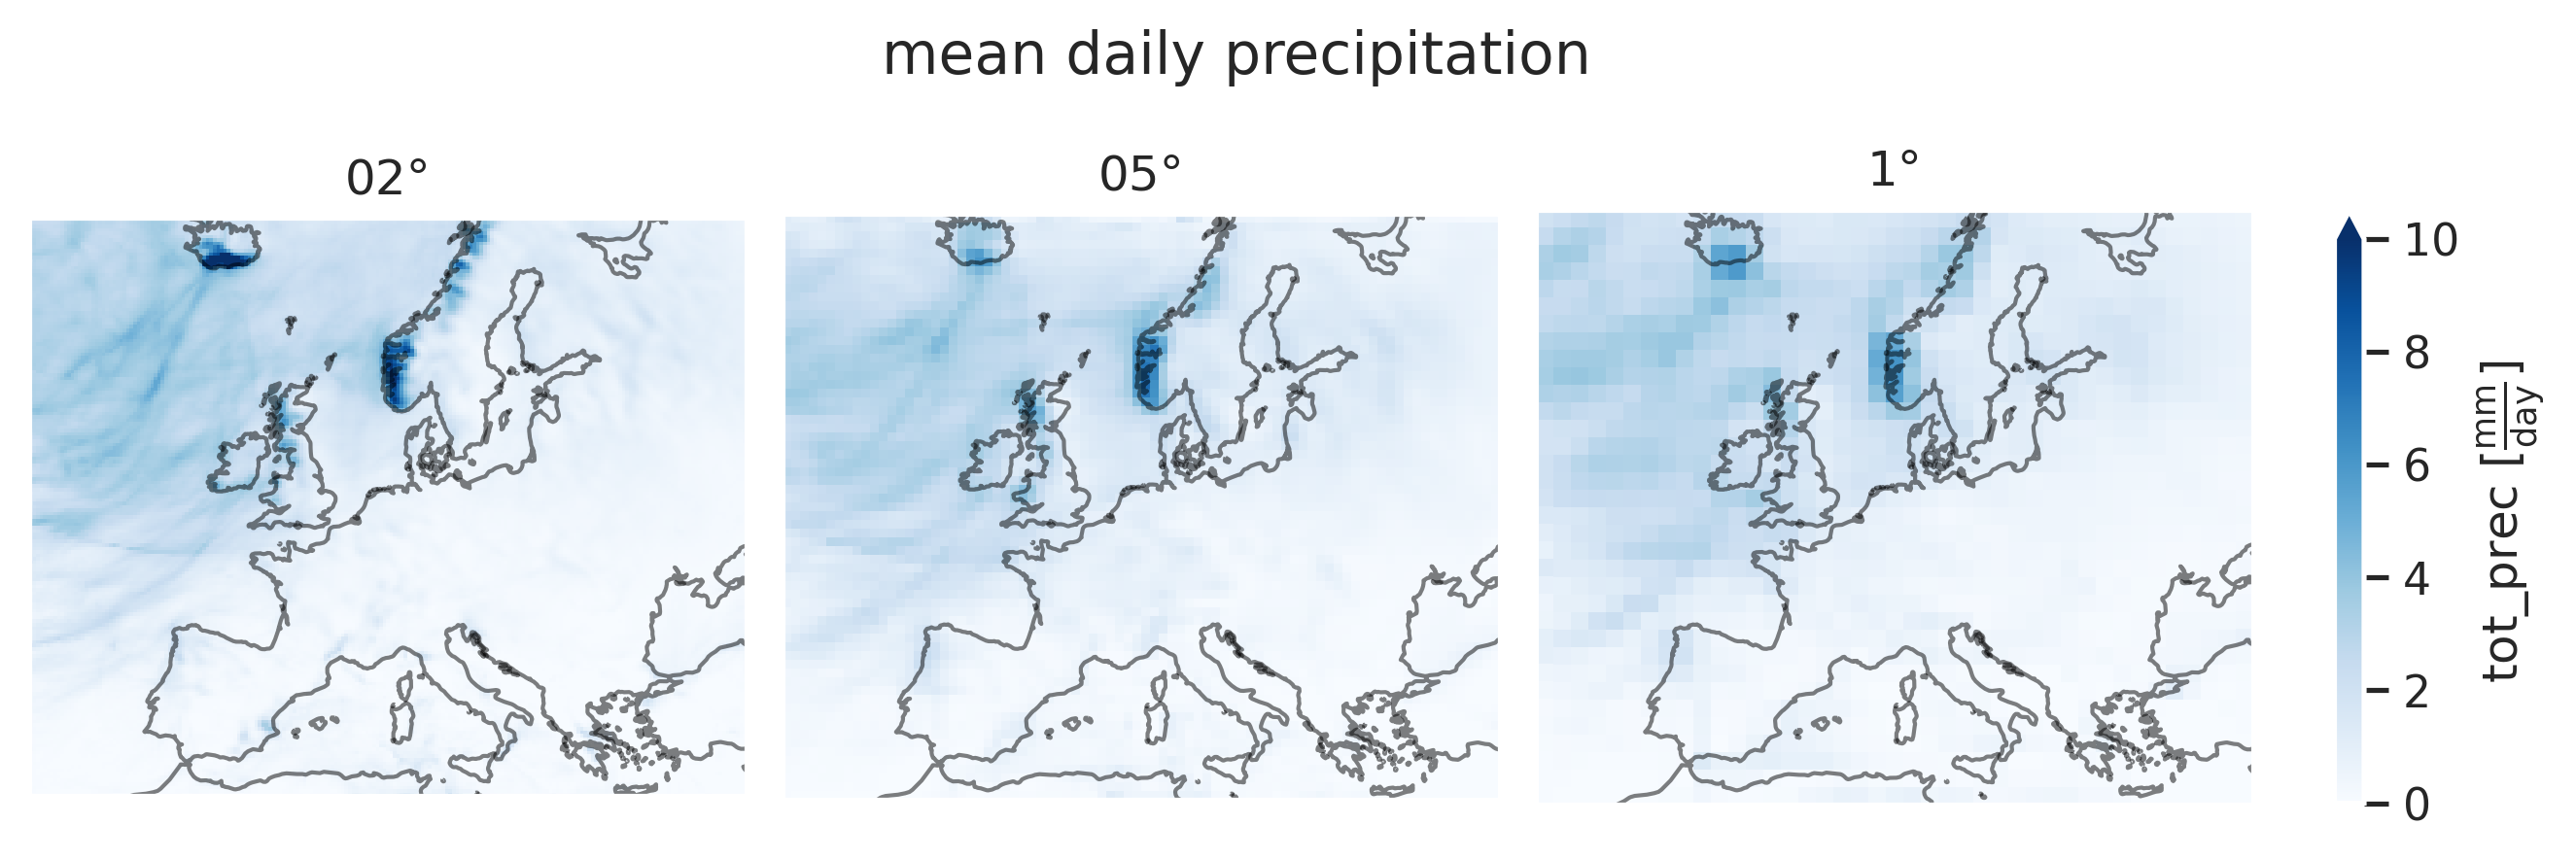
\includegraphics[width=\figwidth]{../figs/2-timmean.png}
	\caption{Temporal mean of daily precipitation sum for different grid resolutions. Simulations ran throughout January 1990.}
	\label{fig:timmean}
\end{figure}

\Cref{fig:timmean} illustrates the spatial distribution of mean precipitation: The general pattern of different grid resolutions is similar, depicting high precipitation rates over the Northern Atlantic and at the coasts of Iceland, Norway and Scotland. However, it is evident that high grid resolution locally increases the intensity of precipitation.

\begin{figure}
	\centering
	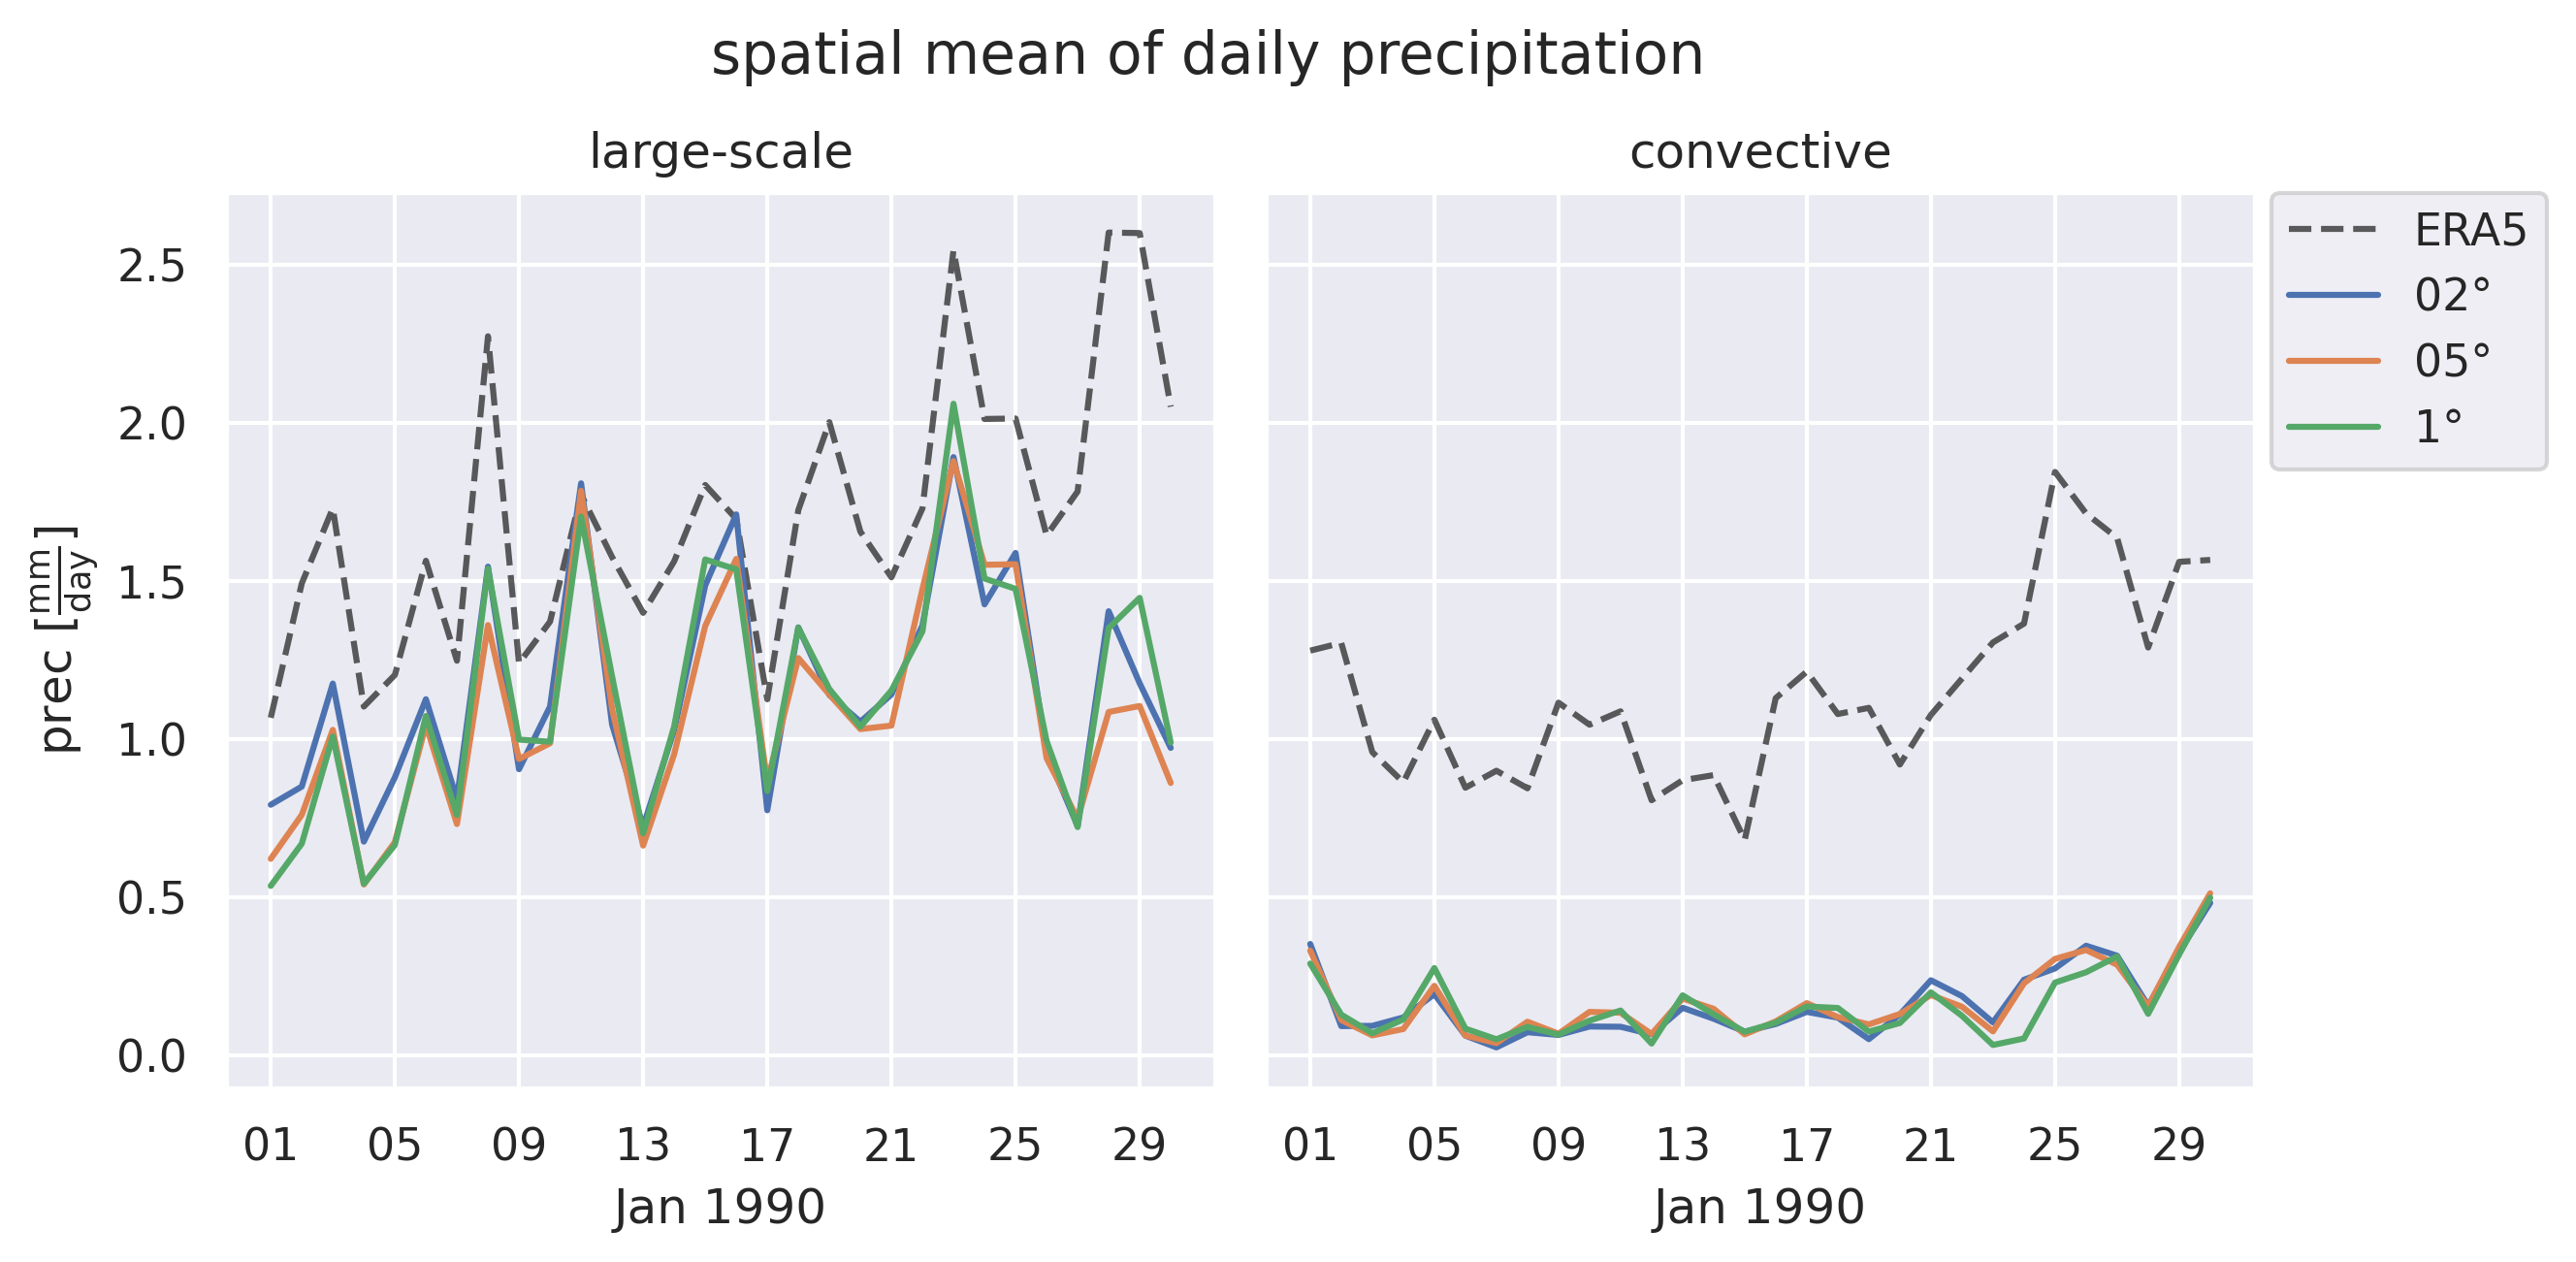
\includegraphics[width=\figwidth]{../figs/5-gsp-con.png}
	\caption{Spatial mean of daily precipitation sum split into large-scale (i.e., grid-scale) and convective signal for different grid resolutions. ERA5 reanalysis data as reference.}
	\label{fig:fldmean}
\end{figure}

When focussing on the temporal domain, the daily precipitation signals of the COSMO-CLM simulations are---generally speaking---similar, indicating that the daily sum over the entire (cropped) model region does not change considerably with model resolution. In \cref{fig:fldmean}, precipitation is split into a grid-scale and convective component, and ERA5 data is included as a reference.
In both subplots, simulations underestimate the observed daily precipitation sum, although the difference between reference and simulation is more pronounced for convective precipitation. The underlying trend in reference and simulation of grid-scale precipitation is comparable, which validates the model results on broader scales. It is important to note though that the simulations have been driven with ERA-Interim data and are now compared to ERA5 data, which might introduce additional biases triggered by different data assimilation procedures of the reanalyses.

The \textit{absolute} difference in precipitation between grid resolutions is more pronounced in the grid-scale precipitation, although without a consistent signal. E.g., in the beginning of January, 0.2°-resolution shows more grid-scale precipitation compared to the remaining resolutions, in the end of the month though, 0.2°- and 1°-resolution show a similar signal, while 0.5°-resolution simulates less grid-scale precipitation. In contrast, variation in the convective part is relatively small. I figure that the missing deep convection scheme is the reason, since all convective precipitation is derived from vertical turbulence only.

\begin{figure}
	\centering
	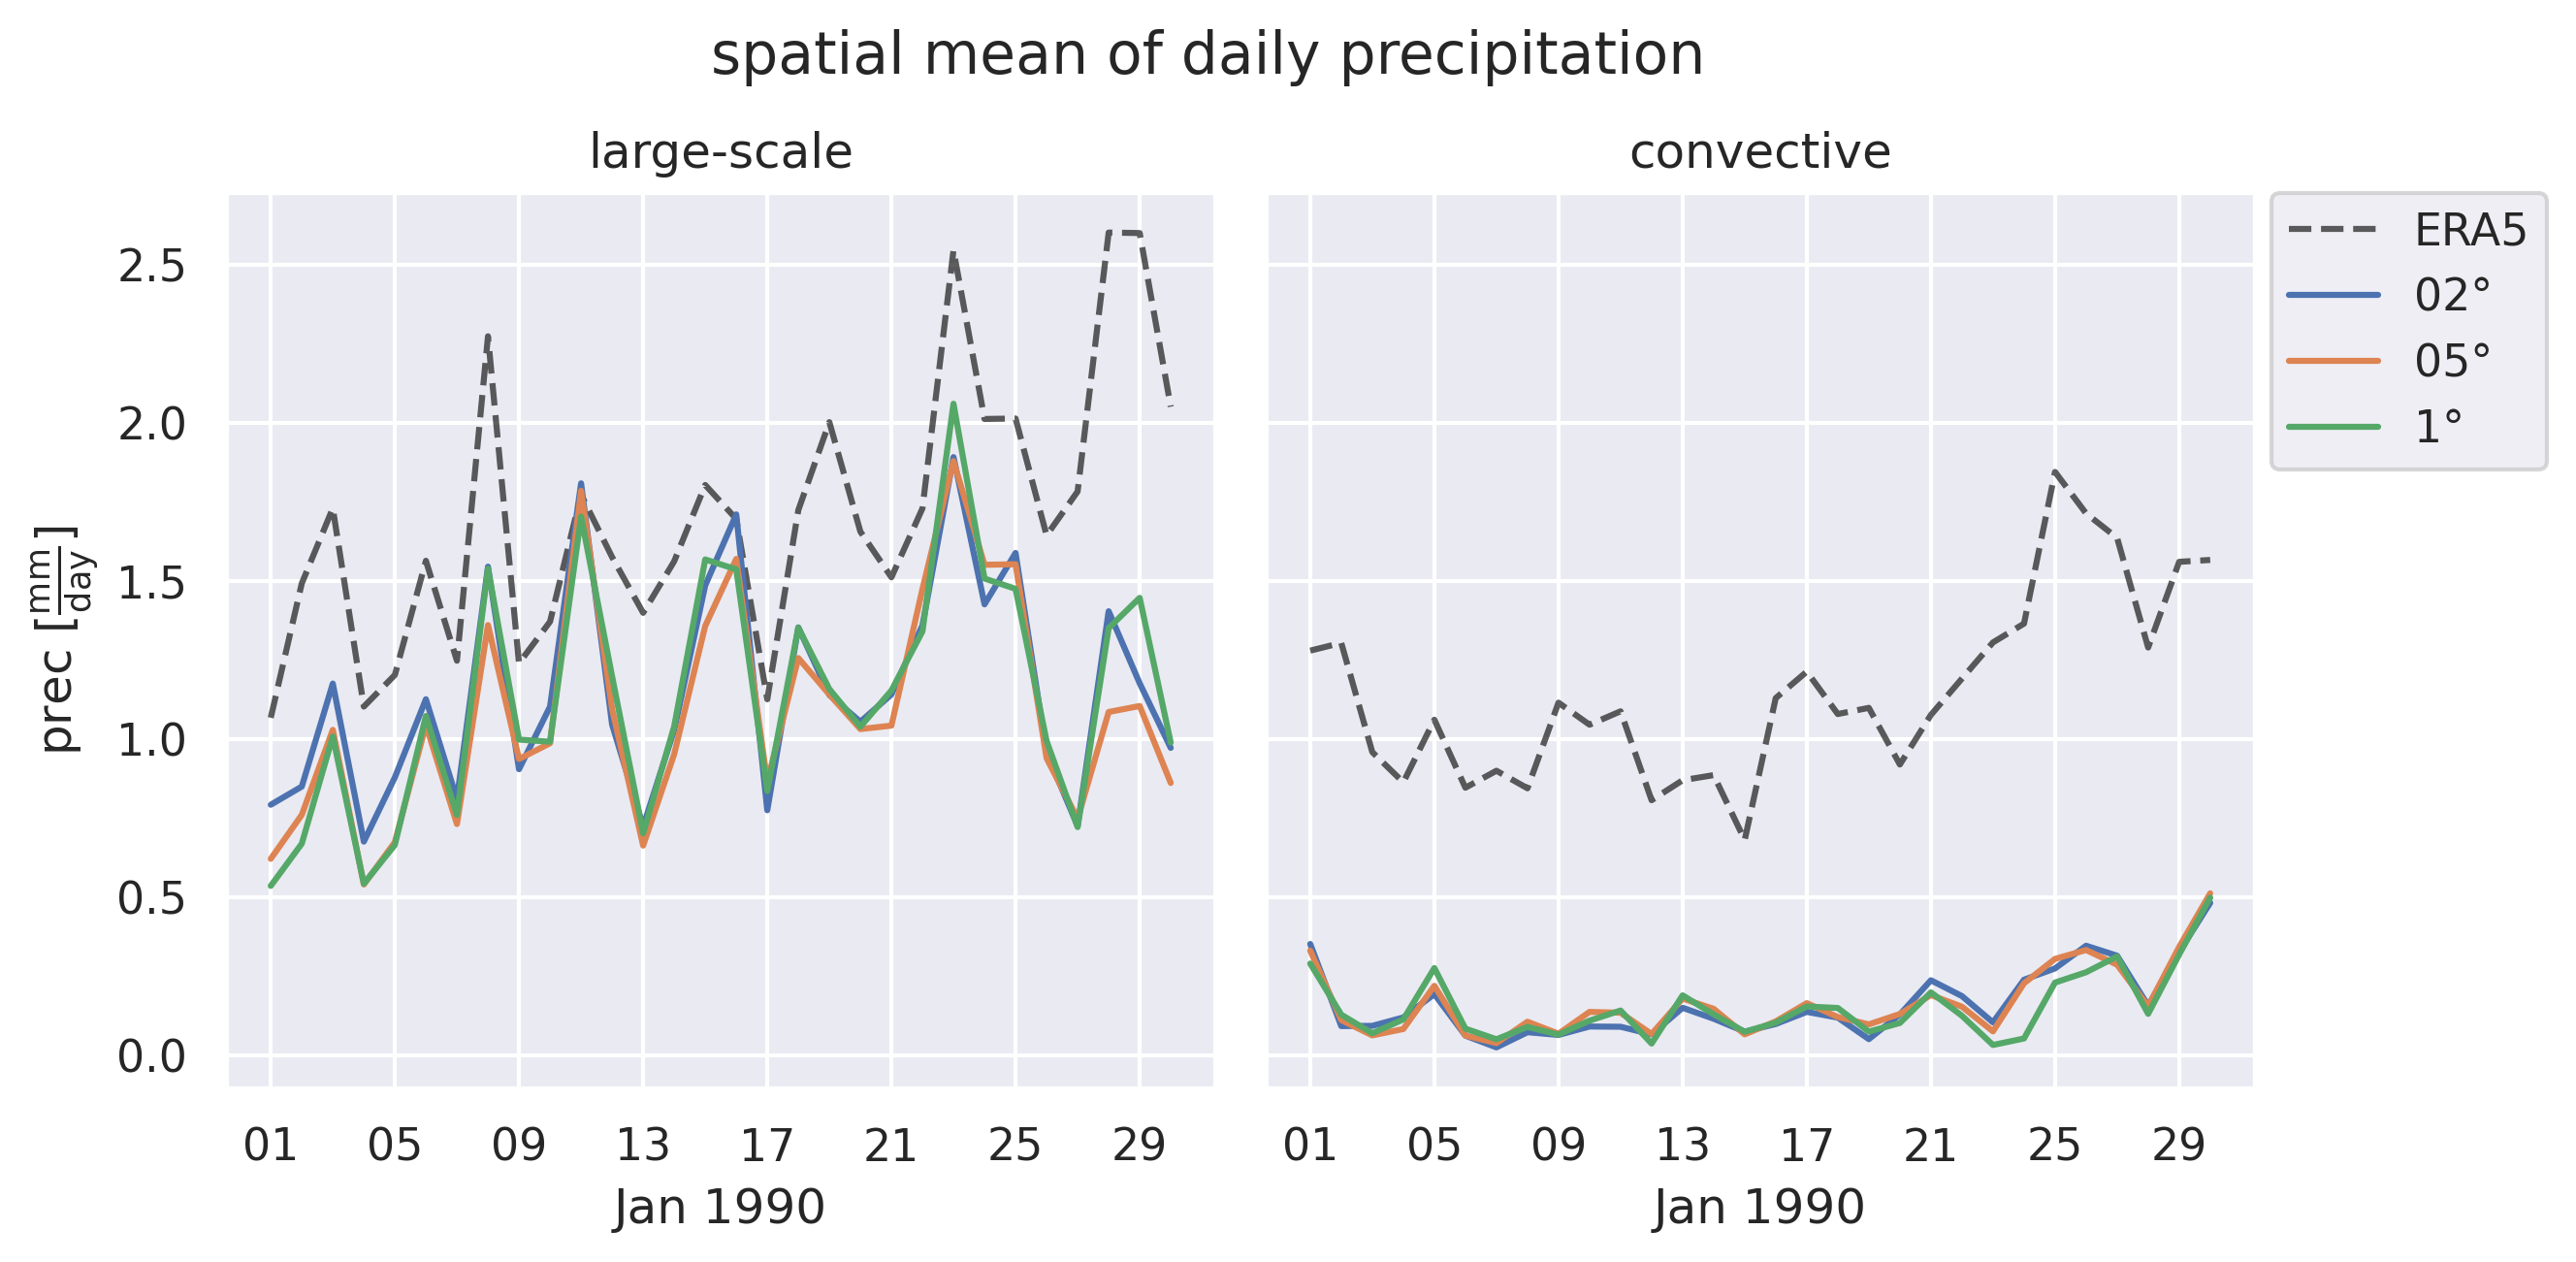
\includegraphics[width=\figwidth]{../figs/5-gsp-con.png}
	\caption{Spatial mean of daily precipitation sum split into large-scale (i.e., grid-scale) and convective signal for different grid resolutions. ERA5 reanalysis data as reference.}
	\label{fig:fldmean}
\end{figure}
	\section{Discussion \& Outlook}

Naturally, high grid resolution improves localization of the precipitation signal, hence, differences in precipitation intensity are visible on maps, but disappear when averaging over all grid boxes. Better localization of precipitation events implies higher number of grid boxes without precipitation, which diminishes the signal when averaging. 

% When localisierung wichtig ist, kleine Gittergröße, aber mean precipitation bleibt auch schon bei geringer auflösung gleich.
	
	\newpage
	\begingroup
	\setlength{\emergencystretch}{3em}
	\printbibliography
	\endgroup
	
	%\newpage
	%\appendix
	%\section{Supplementary material}\label{sec:app}

\begin{figure}[h]
	\centering
	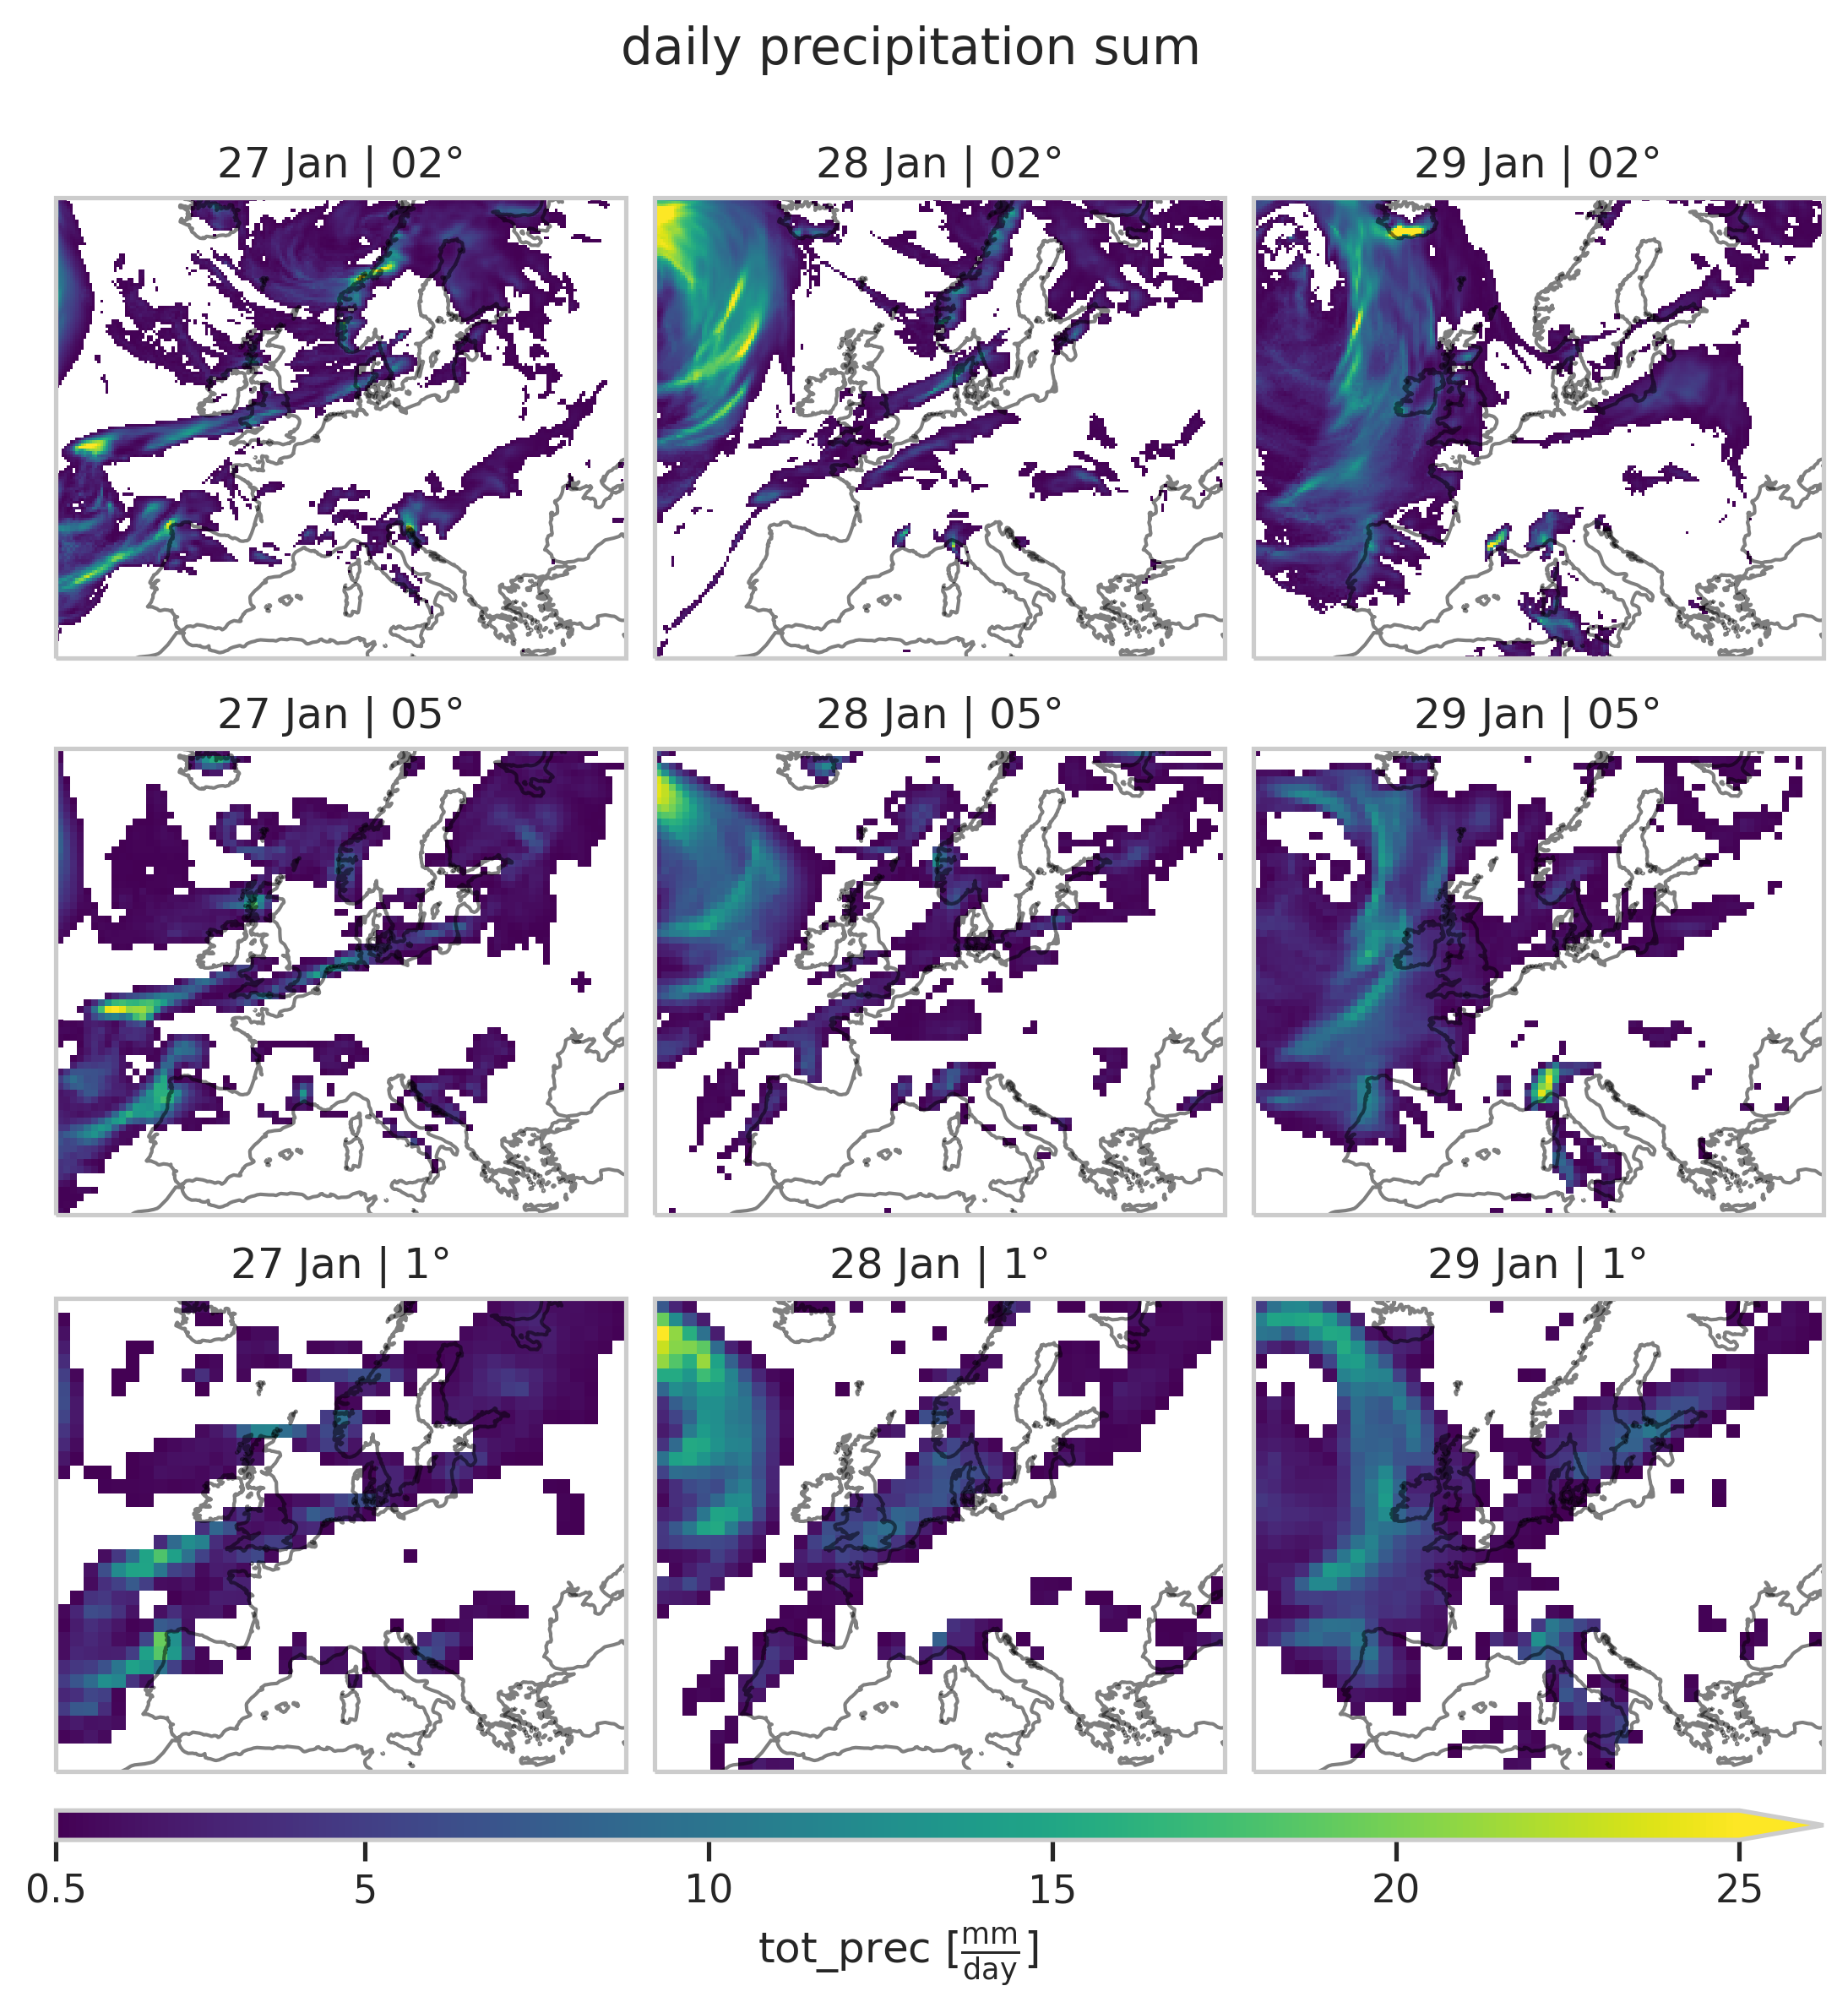
\includegraphics[width=0.7\figwidth]{../figs/6-event.png}
	\caption{Maps of daily precipitation sum during event from 27 to 29 Jan (shortly after \href{https://en.wikipedia.org/wiki/Burns\%27_Day_Storm}{Cyclone \textit{Daria}}). Identical grid resolutions are displayed row-wise, while columns represent single days. Precipitation below \SI{0.5}{\mm\per\day} is excluded. When focussing on the differences among grid resolutions, it is notable that (a) 1°-resolution displays large areas of precipitation in Northeastern Europe, while (b) 0.2°-resolution rather shows high intensities over the Atlantic Ocean and Iceland. Interestingly, solely 0.5°-resolution captures \textit{strong} precipitation event over south-western Alps on 29 Jan, which indicates the complexity of assessing effects of changing grid resolution.}
	\label{fig:app-event}
\end{figure}
	
\end{document}